\documentclass[12pt,a4paper,oneside]{report}
\usepackage[utf8]{inputenc}
\raggedbottom
\sloppy
\usepackage{amsmath}
\usepackage{amsfonts}
\usepackage{amssymb}
\usepackage{ragged2e}
\usepackage{titlesec, soul, tabto,seqsplit}
\usepackage[hidelinks]{hyperref}
\usepackage{caption, subcaption}
\usepackage{graphicx, float, wrapfig, color, mdframed, tabu,tabularx,float}
\usepackage[framed]{matlab-prettifier}
\usepackage[toc,page]{appendix}
\titleformat{\chapter}{\normalfont\huge\bf}{\thechapter.}{20pt}{\huge\bf}
\DeclareRobustCommand{\hlred}[1]{{\sethlcolor{red!20}\hl{#1}}}


\begin{document}


\begin{titlepage}
    \begin{center}
        \vspace*{3cm}  
        {\LARGE
        \textbf{User Guide:\\ \vspace{5mm} RTDD Log Viewer}} 
        \vspace{1.5cm}
        
        \textbf{Anisa Noor Corina}
        
        \vfill
        
        Norwegian University of Science and Technology\\
        Department of Petroleum Engineering and Applied Geophysics\\
        \today
       
    \end{center}
\end{titlepage}

\addcontentsline{toc}{section}{Preface}
\section*{Preface}
This user guide is created to help users to get familiar with the RTDD log viewer program and application. The developers  expect that users can improve the program by reporting bugs and updating the worksheets; \texttt{List Canonical Mnemonic.xlsx} and \texttt{Unit Conversion.xlsx}.
The version 1.0 of RTDD log viewer was developed by Anisa N Corina, Isak Swahn, Sigve Hovda, and Pål Skalle.

The program is also a combination with SeisLab 3.01, copyright{\textsuperscript\textcopyright} 2010, Eike Rietsch, 
copyright {\textsuperscript\textcopyright} 2005, Primoz Cermelj, copyright {\textsuperscript\textcopyright} 2016, The MathWorks, Inc., copyright {\textsuperscript\textcopyright} 2016, MathWorks. All rights reserved.


\chapter{Introduction}
This document contains information regarding the RTDD Log Viewer. RTDD Log Viewer is a program containing source codes that can be compiled to run the application to read real-time drilling data (RTDD). The goal of this application is to provide a user interface enabling user to load and visualize RTDD logging data.

\section{Organization of the manual}
The user manual consists of four main sections: \emph{introduction, system requirements, getting started} and \emph{user interface basis}.
\begin{enumerate}
\item \textbf{Introduction} provides information of the system and its purpose in general terms.
\item \textbf{System requirements} provides a general overview of the system requirement to compile and run RTDD Log Viewer.
\item \textbf{Getting started} explains how to prepare the RTDD Log Viewer program before compiling and prepare a template for plotting the curves.
\item \textbf{RTDD log viewer application} explains the components and features of the viewer application so users getting familiar and enable to run the software quickly.
\item \textbf{Examples of plotting templates} shows some examples of well log plots based on plotting template.
\end{enumerate}

In the appendix, user can find the additional information:
\begin{enumerate}
\item Appendix A: Parsing process
\item Appendix B: Standard format of LAS file
\item Appendix C: Standard format of CSV file
\item Appendix D: Standard format of ASC file
\end{enumerate} 
  
\chapter{System requirements}
The required tool to compile and run this software is MATLAB. The recommended MATLAB version is R2016a, but \emph{any compatibility issues may encountered in older version}. The system requirement of MATLAB R2016a can be found in \url{http://se.mathworks.com/support/sysreq/current_release/} and for the older version in \url{http://se.mathworks.com/support/sysreq/previous_releases.html}. The requirements are also provided in operating systems Windows, Mac, and Linux. The users are expected to have a basic knowledge of coding in MATLAB to get familiar with the program.

\chapter{Getting started}
\section{Download the RTDD log viewer}
The RTDD Log Viewer program can be downloaded in server \texttt{\textbackslash\textbackslash iipt-studio.ivt.ntnu.no\textbackslash drilldb\$}. The RTDD Log Viewer directory is composed of several directories:
\begin{itemize}
\setlength\itemsep{0.1em}
\item log$\_$viewer: Source code of RTDD log viewer.
\item examples: Examples of log data and some templates to plot the track.
\end{itemize}

\section{Compiling RTDD log viewer}
The interface of RTDD Log Viewer is contained in MATLAB code \texttt{main$\_$log.m} and MATLAB figure \texttt{main$\_$log.fig} which located in directory \texttt{log$\_$viewer}. The RTDD log viewer application is opened by compiling the \texttt{main$\_$log.m} in MATLAB. To compile the RTDD log viewer:
\begin{enumerate}
\item Open \texttt{main$\_$log.m}
\item Press run button or F5
\item The user interface of RTDD log viewer will appear in a new window
\end{enumerate}

\section{Preparing the plotting template}
\label{ch:plot_template}
In order to show the log curves in the application, user is required to write source codes determining the input of plotting template. Some plotting templates are ready to be used in directory \texttt{example}. A plotting template must contain information of the log tracks and log curves which are written as input: \texttt{inputTrack} and \texttt{inputCurve}.

\subsection{Writing input for \texttt{inputTrack}}
\label{ch:input_track}
\texttt{inputTrack} is a variable with class of \texttt{struct}\footnote{http://se.mathworks.com/help/matlab/ref/struct.html}. This variable contains all the information regarding the track properties: name, plotted curves, and the scale of the axes. All these information are defined in fields of \texttt{inputTrack} structure,
\begin{description}
\item[\texttt{inputTrack.Name}] specifies the log track to be plotted and the track name. There is no limitation of the number of the tracks to be plotted. The input can be written as: \texttt{inputTrack.Name = \{'<track $\#1$>','<track $\#2$>',...\}}

\item[\texttt{inputTrack.Curves}] contains the canonical name of curves which is assigned in each particular track. The canonical name is the default name of log curves that acknowledged by the RTDD program. This is constructed due to a large number of curves mnemonic name which are varies within each service company. The list of canonical and mnemonic name are saved in a worksheet \texttt{List Canonical Mnemonic.xlsx} in directory \texttt{log$\_$viewer}. There can be multiple curves plotted in one track up until 5 curves. The input can be written as:

\texttt{inputTrack.Curves= \{\{'<can.name $\#1$>','<can.name $\#2$>'\}, \{'<can.name $\#1$>'\}...\}}

\item[\texttt{inputTrack.XScale}] contains the scale of values along the x-axes. The input must be in 'linear' or 'log'. The 'linear' input set the curves in the corresponding track to be plotted in a linear x-scale, while 'log' input plots the curve in a logarithmic x-scale. The inpit can be written as:
\texttt{inputTrack.Curves= \{'linear'|'log',...\}}

\noindent \textbf{Note:} It is not suggested to assign log curves that are supposed to be plotted in logarithmic scale (logarithmic log curves) and linear log curves together in one track. For example, resistivity log is suggested to be plotted in separate logarithmic track.
\end{description}

An example of input of \texttt{inputTrack} below shows that there are 3 tracks to be plotted, Track 1, Track 2, and Track 3. Track 1 has 2 curves, hookload and WOB, while each Track 2 and Track 3 has 1 curve, SPP and BPOS curve consecutively.
\pagebreak

\begin{lstlisting}[style=Matlab-editor]
inputTrack = struct(...
    'Name',{'Track 1','Track 2','Track 3'},...
    'Curves',{{'HKLD','WOB'},...
    	     {'SPP'},...
    	     {'BPOS'}},...
    'XScale',{'linear','linear','linear'});
\end{lstlisting}

\paragraph{}
\begin{wrapfigure}[7]{l}{0.1\textwidth}
\vspace{-15pt}

\includegraphics[scale=0.03]{light_bulb.jpg}
\end{wrapfigure}
\noindent\textbf{Note:} The program can be forced to acknowledge curve which is not listed in the \texttt{List Canonical Mnemonic.xlsx}. As an example, if user want to plot STICK$\_$RT, which is not listed in the worksheet, the user can set 'STICK$\_$RT' in \texttt{inputTrack.Curves}. Then, the program will be forced to acknowledge STICK$\_$RT curve in the log file and plot it. However, it is recommended to add the mnemonic name which is not listed into the worksheet.

\subsection{Writing input for \texttt{inputCurves}}
\texttt{inputCurves} is an input variable with class of \texttt{struct} which contains information of the curves properties to be plotted. The properties that can be set include curve line width, log curve range value, curve line color, and curve units. All these information are defined in fields of \texttt{inputCurves} structure,
\begin{description}
\item[\texttt{inputCurves.Name}] contains the canonical name of the curves based on the curve name in input \texttt{inputTrack}. This input \textbf{must be written as the first field}. The input can be written:

\texttt{inputCurves.Name = \{'<canonical name $\#$1>','<canonical name $\#$2>',...\}}

\item[\texttt{inputCurves.Unit}] contains the unit of the curves that user desired. By changing the curve unit, the curve unit from the log file will be converted to the new input. If the user set the input with 'auto', the curve unit from the log file will be converted to the default unit. The default unit of log curves can be found in worksheet \texttt{List Canonical Mnemonic.xlsx} and the list of units are collected in worksheet \texttt{Unit Conversion.xlsx}.The input can be written:

\texttt{inputCurves.Unit = \{'<unit in string>'|'auto',...\}}


\noindent\textbf{Note:} It is suggested for user to write the unit input following the list in  worksheet \texttt{Unit Conversion.xlsx} because the conversion process is case sensitive.

\item[\texttt{inputCurves.Min}] contains the minimum value of the curves. If this variable is set to 'auto', the program will automatically set the default value. The input can be written:

\texttt{inputCurves.Min = \{<numeric value>|'auto',...\}}

\item[\texttt{inputCurves.Max}] contains the maximum value of the curves. If this variable is set to 'auto', the program will automatically set the default value. The input can be written:

\texttt{inputCurves.Max = \{<numeric value>|'auto',...\}}

\item[\texttt{inputCurves.LineWidth}] contains the line width value. If this variable is set to 'auto', the curves are plotted with 0.5 points. The input can be written:

\texttt{inputCurves.LineWidth = \{<numeric value>|'auto',...\}}

\item[\texttt{inputCurves.LineColor}] contains the line color of the curves. The input must be in RGB triplet, a three-element row vector whose elements specify the intensities of the red, green, and blue components of the color. The intensities must be in the range [0,1]. If this variable is set to 'auto', the curves are plotted following the default colors.

\texttt{inputCurves.LineColor = \{<RGB triplet>|'auto',...\}}

\end{description}

These curve properties are optional, if user don't want to change the default curve properties, this input variable can be set as an empty matrix, \texttt{inputCurves=[]}. User can decide which curve properties to be changed. An example of \texttt{inputCurves} is shown below. This input follows the example of input \texttt{inputTracks} in \hyperref[ch:input_track]{Chapter \ref{ch:input_track}}. The input in example shows that user change the properties of curves HKLD and SPP without changing the properties of curves WOB and BPOS.
\begin{lstlisting}[style=Matlab-editor]
inputCurves = struct('Name',{'HKLD','SPP'},...
    'Unit',{'KGFM','bar'},...
    'Min',{'auto',0,},...
    'Max',{200000,'auto'},...
    'LineWidth',{'auto',0.8},...
    'LineColor',{[0.000,  0.447,  0.741],[0.800,  0.000,  0.200]});
\end{lstlisting}

\pagebreak
\begin{wrapfigure}[6]{l}{0.1\textwidth}

\includegraphics[scale=0.03]{light_bulb.jpg}
\end{wrapfigure}
\noindent\textbf{Suggestion:} If user only want to change only several properties, example \texttt{Min} and \texttt{Max} properties of the curves, user can remove the other unnecessary fields. Example:
\begin{lstlisting}[style=Matlab-editor]
inputCurves = struct('Name',{'HKLD','SPP'},...
    'Min',{'auto',0,},...
    'Max',{200000,'auto'});
\end{lstlisting}

\chapter{RTDD log viewer application: user interface basis}
\section{RTDD log viewer application user interface}
After compiling the source code, RTDD log viewer application will appear in a window. The components and terms of the interface is shown in \hyperref[fig:full_window]{Fig. ~\ref{fig:full_window}}.
\begin{figure}[h]
\centering
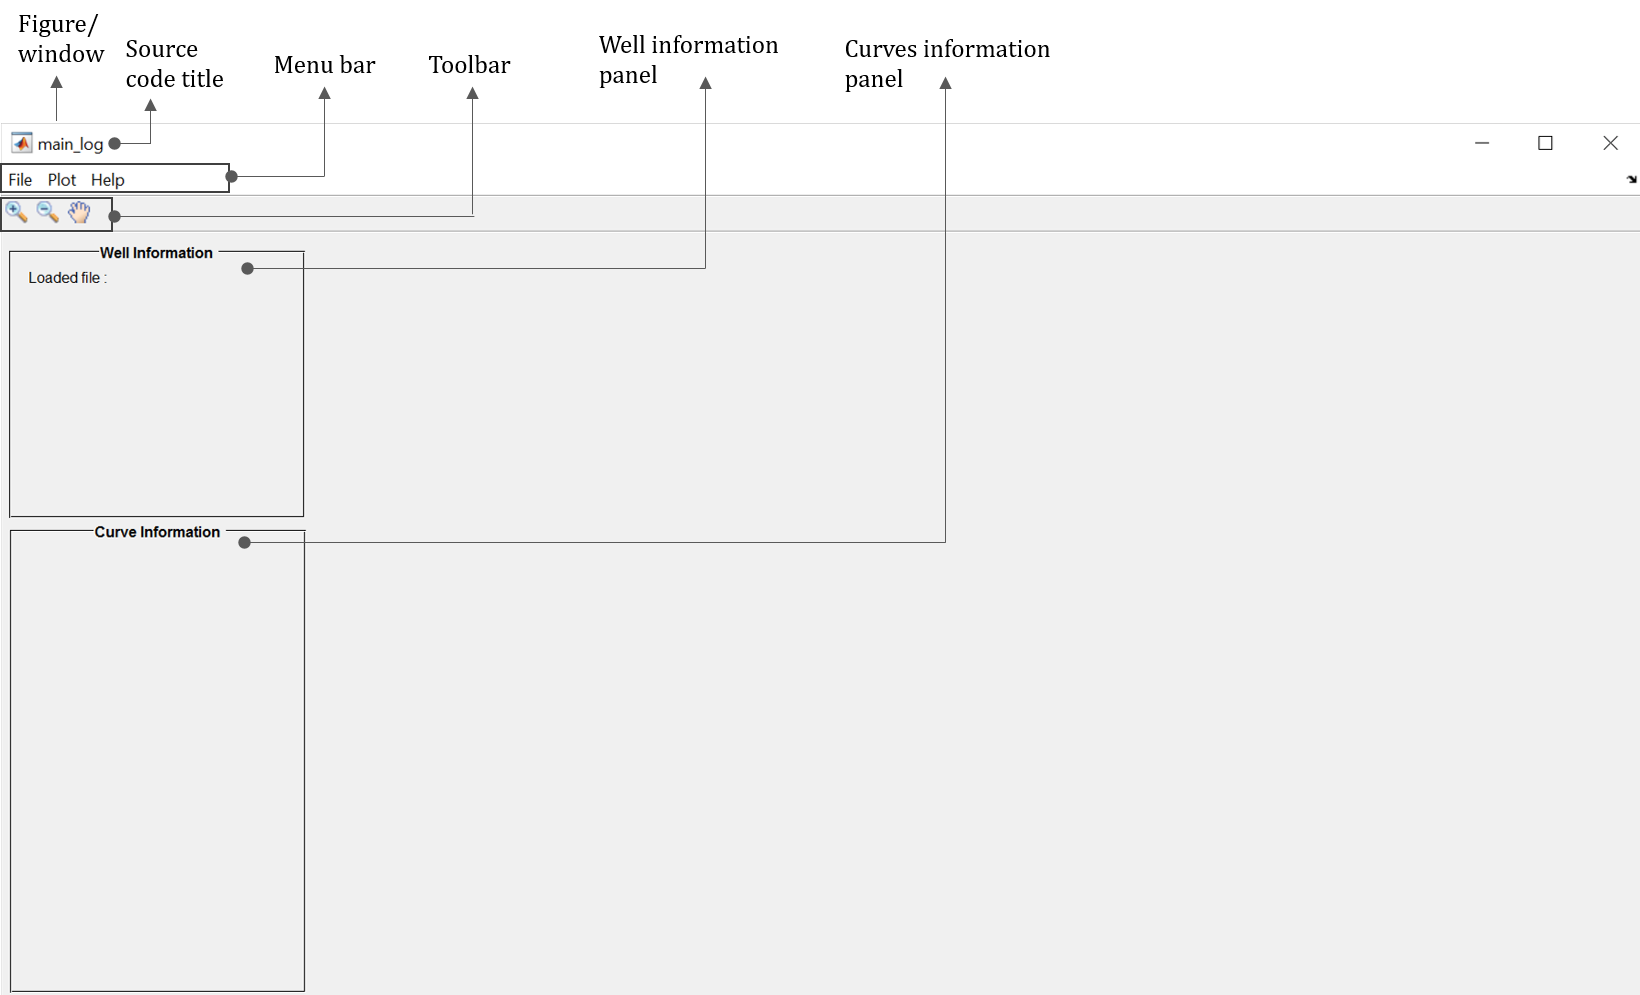
\includegraphics[width=1\textwidth]{full_win_desc.png}
\caption{Full window of log viewer application}
\label{fig:full_window}
\end{figure}

\subsection{Menu bar}
The RTDD log viewer application contains a pull-down menu bar so user can access the features of the application. The menu bar contains:
\begin{description}
\item[File] menu provides an option to load the preferred files.
\item[Plot] menu provides an option to plot the loaded file based on the selected template.
\item[Help] menu provides option to open the user manual or show the information of the application.
\end{description}


\subsection{Toolbar}
\begin{wrapfigure}[2]{l}{0.05\textwidth}
\vspace{-15pt}

\includegraphics[scale=1]{scopes_button_pan.png}
\end{wrapfigure}
\textbf{Pan tool} activates mouse-based panning for any axes in the current figure.

\begin{wrapfigure}{l}{0.05\textwidth}
\vspace{-15pt}

\includegraphics[scale=0.9]{tool_zoom_in.png}
\end{wrapfigure}
\noindent \textbf{Zoom in tool} activates interactive zooming into the point beneath the mouse for any axes in the figure.

\begin{wrapfigure}{l}{0.05\textwidth}
\vspace{-15pt}

\includegraphics[scale=0.9]{tool_zoom_out.png}
\end{wrapfigure}
\noindent \textbf{Zoom out tool} activates interactive zooming out from the point beneath the mouse for any axes in the figure.

\subsection{Well information panel}
The well information panel provides information of the log file that successfully loaded into the application and information of the well. The information will appear after user load the file. The information contains:
\begin{itemize}
\setlength\itemsep{0.1em}
\item Loaded file name
\item Well name
\item Well field
\item Well location
\item Country
\item Service: the service company which perform the logging operation
\item Start date: the date and time of logging operation executed
\item Stop date: the date and time of logging operation ended
\end{itemize}

\begin{figure}[h]
\centering
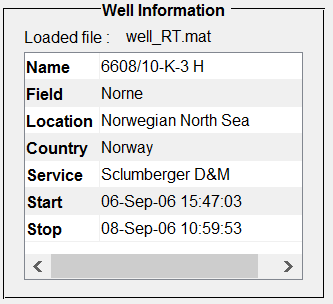
\includegraphics[width=0.4\textwidth]{well_info_panel.PNG}
\caption{Well information panel after load the log file}
\label{fig:well_info_panel}
\end{figure}

\subsection{Curves information panel}
This panel shows the mnemonic names and units of all of the logging curves contained in the log file. This panel will be shown once the file loaded.
\begin{figure}[h!]
\centering
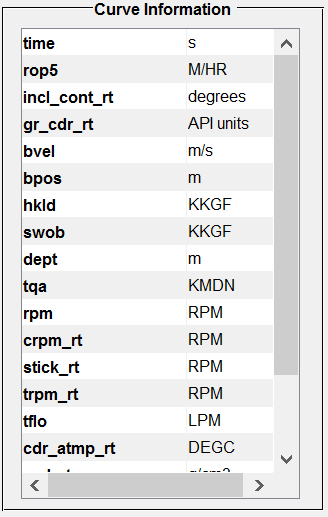
\includegraphics[width=0.5\textwidth]{available_curve_panel.PNG}
\caption{Curve information panel after load the log file}
\label{fig:curve_info_panel}
\end{figure}

\section{Load file into RTDD log viewer}
There are 3 types of log file that can be loaded into the program:
\begin{itemize}
\setlength\itemsep{0.1em}
\item *.las (LAS 2.0 and 3.0)
\item *.csv
\item *.asc
\item *.mat
\end{itemize}

\noindent To load the log file into the application,
\begin{enumerate}
\setlength\itemsep{0.1em}
\item In the menu bar, choose \textbf{File} $>$ \textbf{Load file...}
\item A new window will show up and choose the desired log file (*.las/*.csv/*.mat)
\item Click \textbf{OK} to load.
\end{enumerate}

During loading process, the file is also parsed by the program. The details of parsing process can be found in \hyperref[ch:parsing]{Appendix\ref{ch:parsing}}. In order to avoid errors during parsing, it is very important to check the log file according to the standard format. All the standardized formats for the log file are discussed in \hyperref[ch:las_std]{Appendix \ref{ch:las_std}}, \hyperref[ch:csv_std]{Appendix \ref{ch:csv_std}}, and \hyperref[ch:asc_std]{Appendix \ref{ch:asc_std}}.


\section{Save the parsed file}
\label{ch:save_file}
The output from parsing can be saved in\texttt{.mat} file. To save the file:
\begin{enumerate}
\item In the menu bar, choose \textbf{File $\>$ Save file...}
\item A new window will show up and select the destination folder of the file
\item Click \textbf{Save} to save the file.
\end{enumerate}

\section{Plot log curves in RTDD log viewer}
To plot the curves from the loaded file in the application:
\begin{enumerate}
\item In the menu bar, choose \textbf{Plot} $>$ \textbf{Load template...}
\item Select the plotting template (see \hyperref[ch:plot_template]{Chapter \ref{ch:plot_template}} for information of preparing plotting template)
\item Click \textbf{OK} to plot.
\end{enumerate}

\section{Navigating around RTDD log viewer}
This section provides information of terms and features in RTDD log viewer application after plotting the curves. The components of the applications after the curves plotted are shown in \hyperref[fig:win_w_curves]{Figure \ref{fig:win_w_curves}}.

\begin{figure}[ht]
\centering
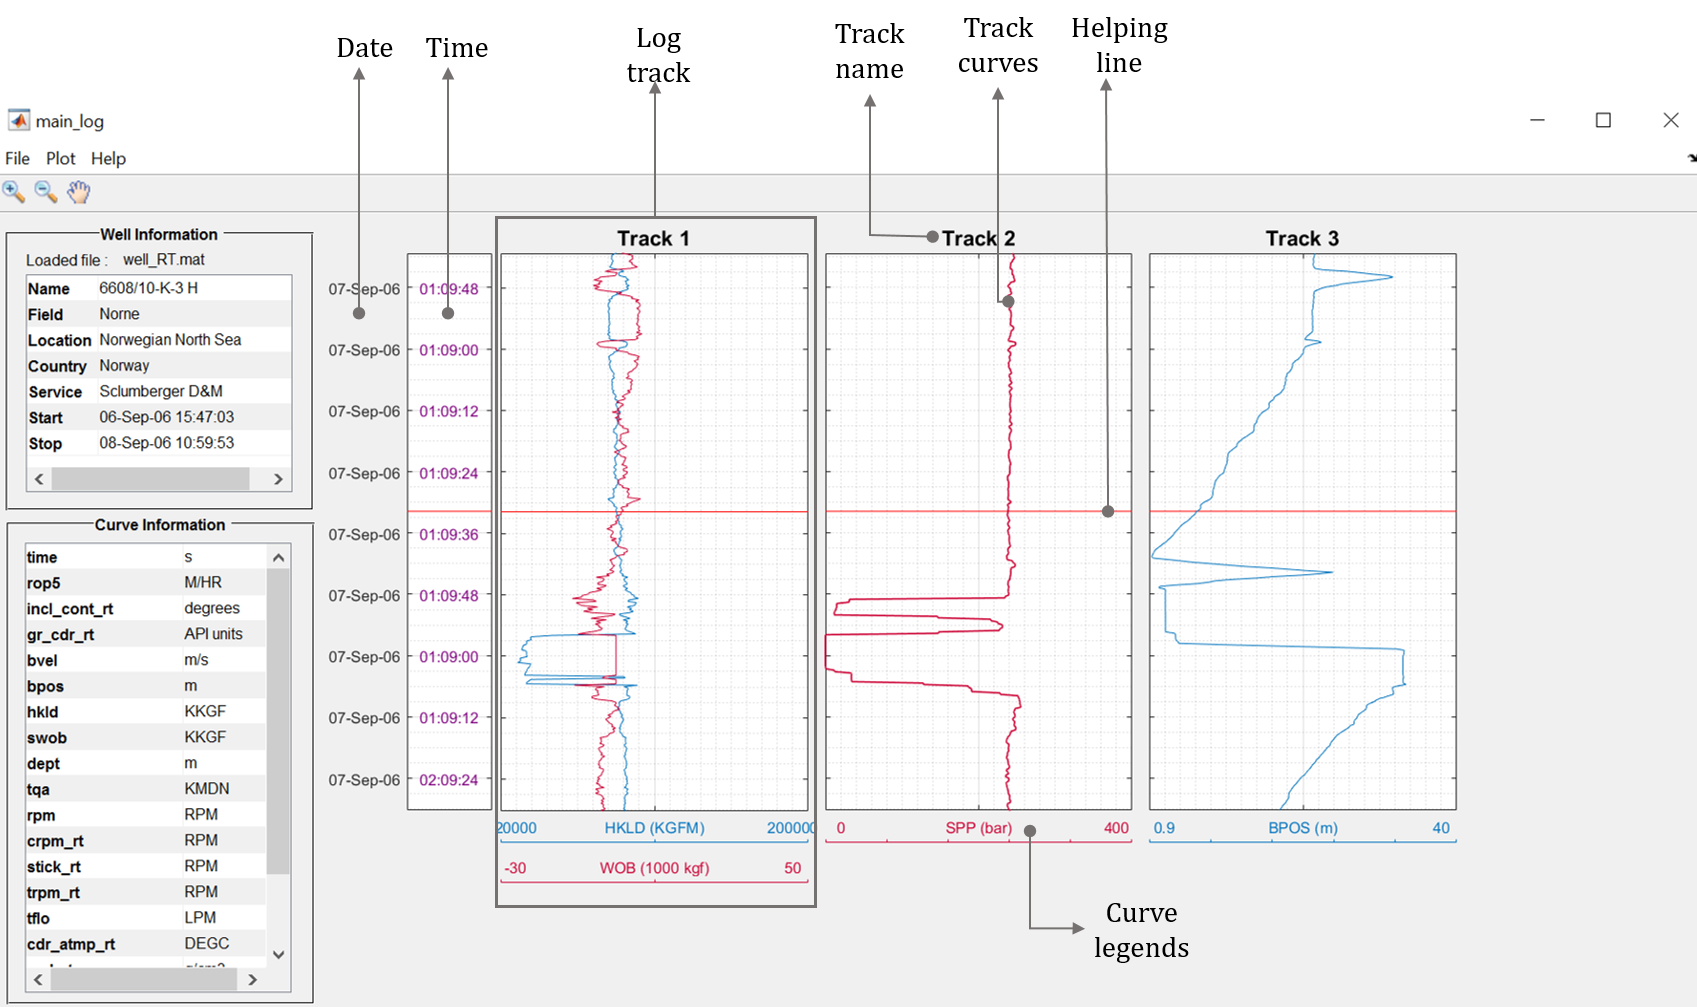
\includegraphics[width=\textwidth]{win_w_curves.png}
\caption{RTDD log viewer after curves plotted}
\label{fig:win_w_curves}
\end{figure}

\begin{description}
\item[Date and time] shows the date and time which are the curves' reference.
\item[Log track] is described as one component which consists of track name, track curves, and track legends.
\item[Track name] shows the tracks' name which is based on the user input.
\item[Track curves] shows the plotted curves which is based on the user input.
\item[Track legends] shows the names, units, and minimum and maximum value of plotted curves.
\end{description}

\noindent Some of the features in RTDD log viewer application.
\begin{enumerate}
\setlength\itemsep{0.1em}
\item{Helping line}
\item{Hide curves feature}
\item{Interactive data cursor}
\item{Track description}
\item{Zoom in and out}
\item{Pan}
\end{enumerate}

\subsection{Helping line}
Helping line is a horizontal line which stretched over date and time axes and all log tracks axes. This helping line is moving interactively as the user move the cursor over the log track axes. The purpose of helping line is to improve reading the curves, especially during comparing curves value. The helping line has red color as can be seen in \hyperref[fig:win_w_curves]{Figure \ref{fig:win_w_curves}}.

\subsection{Hide curves feature}
This feature provides a functionality to hide the curve(s) plotted in a log track. To hide the curve(s),
\begin{enumerate}
\setlength\itemsep{0.1em}
\item Hover the cursor over the legend of the selected curve
\item Click the legend to hide the curve
\item Click the legend again to unhide the curve
\end{enumerate}

\begin{wrapfigure}[2]{l}{0.1\textwidth}
\vspace{-15pt}

\includegraphics[scale=0.08]{hand_point.png}
\end{wrapfigure}
\noindent\textbf{Attention:} This feature can not be processed while \emph{zoom or pan mode} is active.

\begin{figure}[H]
\centering
  \begin{subfigure}[b]{0.31\textwidth}
    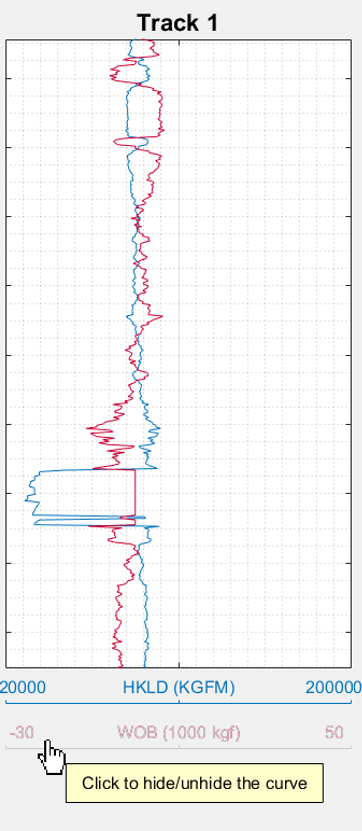
\includegraphics[width=\textwidth]{1_hide.png}
    \caption{}
    \label{fig:f1}
  \end{subfigure}
  \hfill
  \begin{subfigure}[b]{0.31\textwidth}
    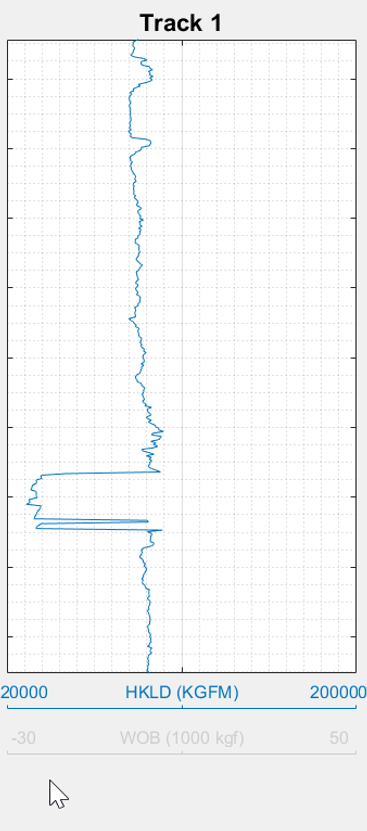
\includegraphics[width=\textwidth]{2_hide.png}
    \caption{}
    \label{fig:f2}
  \end{subfigure}
   \hfill
  \begin{subfigure}[b]{0.31\textwidth}
    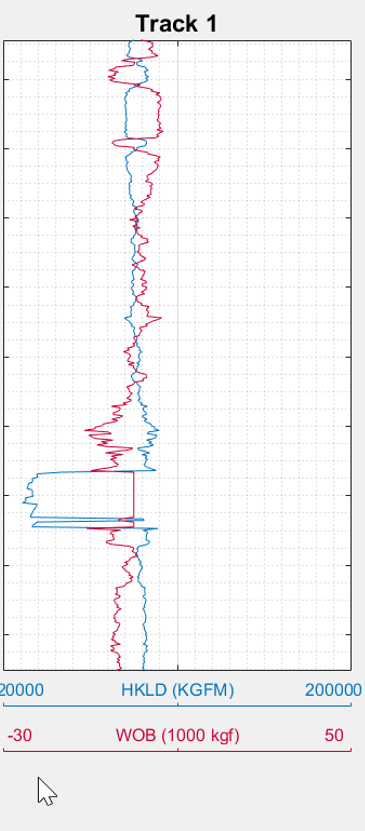
\includegraphics[width=\textwidth]{3_hide.png}
    \caption{}
    \label{fig:f2}
  \end{subfigure}
  \caption{Hide curves feature: (a) Hover cursor over legend, (b) the curves hidden and legend turns to grey color, and (c) unhide the curve by clicking legend again}
  
\end{figure}

\subsection{Interactive data cursor}
This feature provides a functionality to show a data tip. A data tip is a small box that appears when user move the cursor over the line curve and floats within an axes. The data tip display the values of the curve at data cursor location, including the date and time.
\begin{figure}[H]
\centering
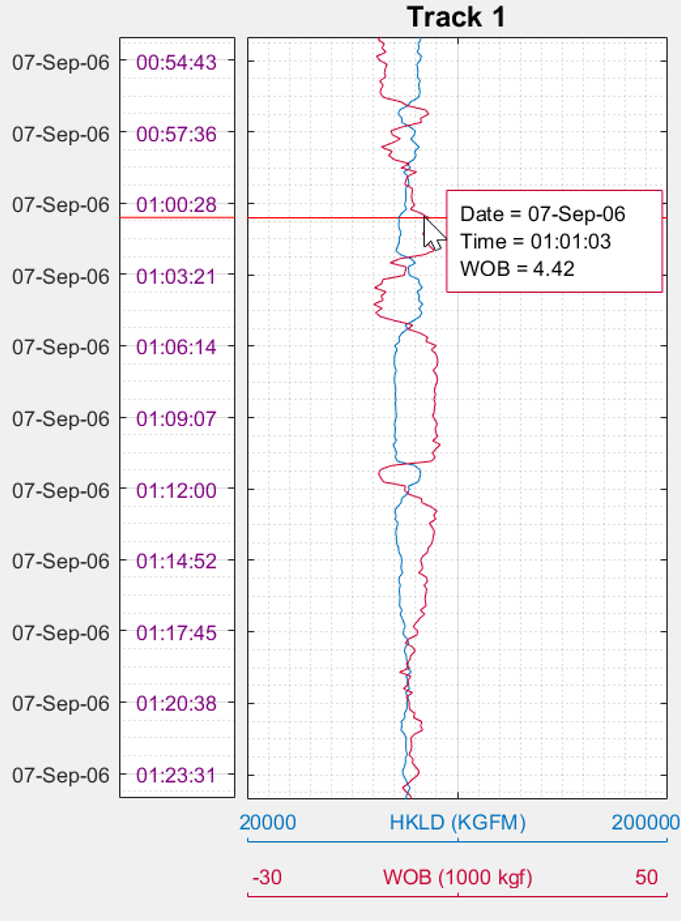
\includegraphics[width=0.6\textwidth]{cursor.png}
\caption{Interactive data cursor and data tip}
\end{figure}

\begin{wrapfigure}[2]{l}{0.1\textwidth}
\vspace{-15pt}

\includegraphics[scale=0.08]{hand_point.png}
\end{wrapfigure}
\noindent\textbf{Attention:} The data tip is not appear when \emph{zoom or pan mode} is active.

\subsection{Track description}
Track description feature provides a description of the curves plotted within the selected track. To view the track description,
\begin{enumerate}
\setlength\itemsep{0.1em}
\item Hover the cursor over the track name
\item Click the track name. Then, a new window will appear
\item Click close to close the track description.
\end{enumerate}

\begin{figure}[H]
\centering
  \begin{subfigure}[b]{0.4\textwidth}
    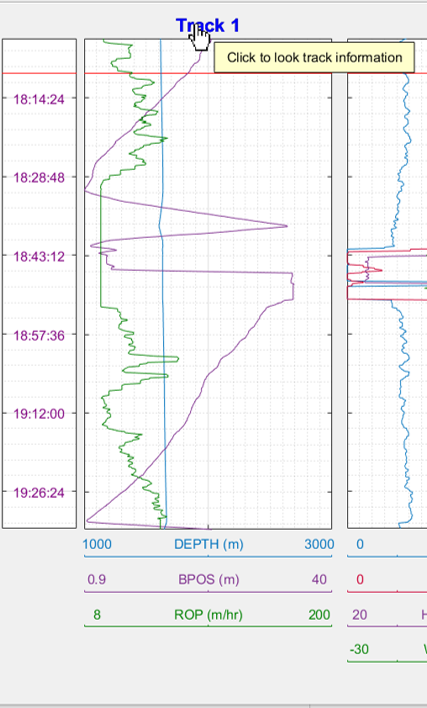
\includegraphics[width=\textwidth]{track_des_1.png}
    \caption{}
  \end{subfigure}
   \hfill
  \begin{subfigure}[b]{0.55\textwidth}
    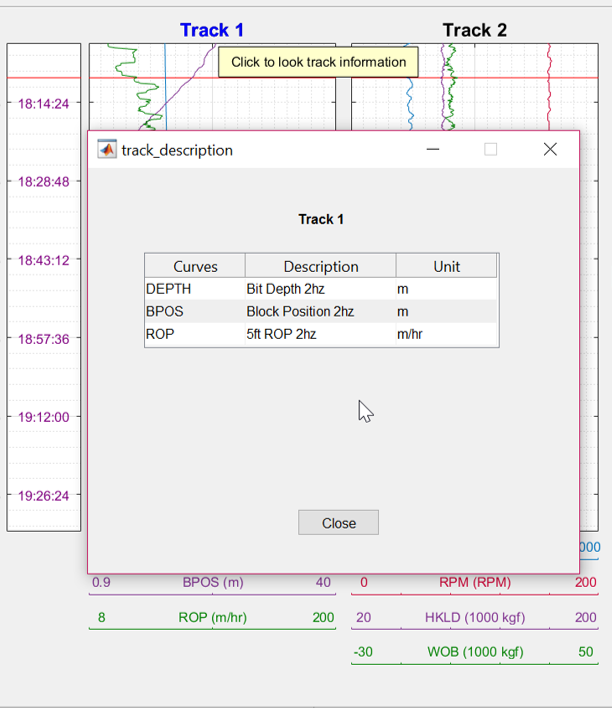
\includegraphics[width=\textwidth]{track_des_2.png}
    \caption{}
  \end{subfigure}
  \caption{Track description features: (a) Click the track name and (b) new window showing track description will appear}
  
\end{figure}



\subsection{Zoom in and out}
Zoom in/out features can be activated by clicking the zoom in/out icon in toolbar. During the zoom in/out mode is active, user can found some options of zoom in/out functionality from the pop-up menu which appears from right-click operation on the axes. In this pop-up menu, user can select zooming motion --- horizontal, vertical, and both direction --- and reset to the original view.

\subsection{Pan}
Pan feature can be activated by clicking the pan icon in the toolbar. During the pan mode is active, user can found some options of pan functionality from the pop-up menu which appears from right-click operation on the axes. In this pop-up menu, user can select panning motion --- horizontal, vertical, and both direction --- and reset to the original view.

\begin{figure}[ht]
\centering
\begin{subfigure}[b]{0.45\textwidth}
    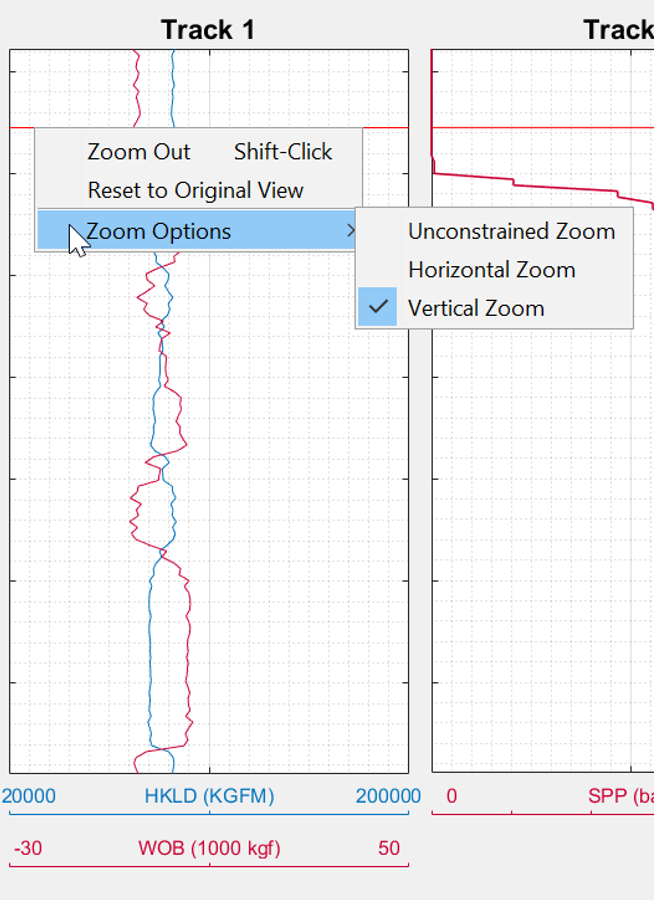
\includegraphics[width=\textwidth]{zoom.png}
    \caption{Options in the pop-up menu during the active zoom in/out mode}
\end{subfigure}
\hfill
  \begin{subfigure}[b]{0.45\textwidth}
    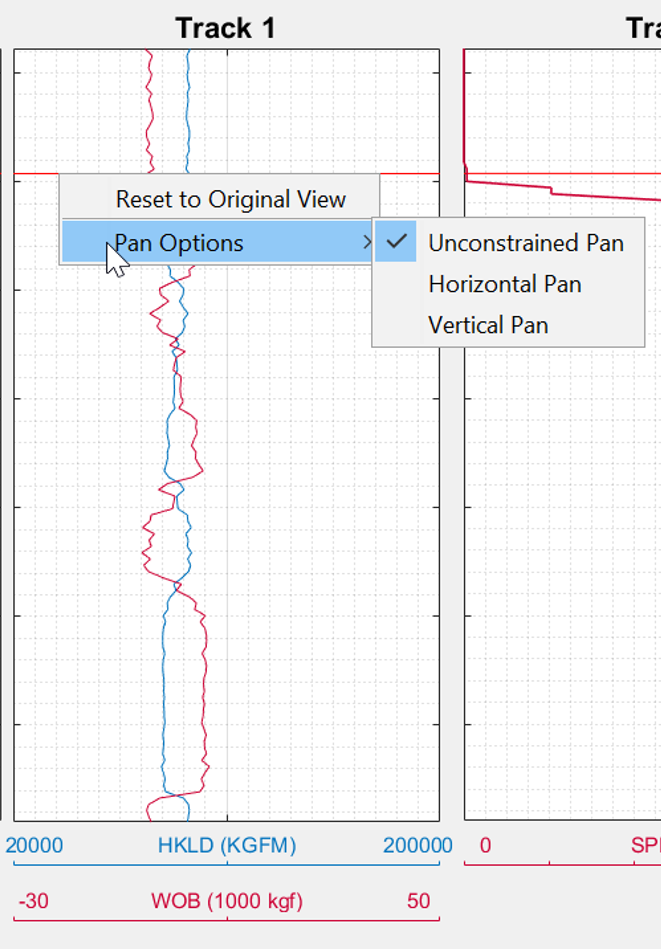
\includegraphics[width=\textwidth]{pan.png}
    \caption{Options in the pop-up menu during the active pan mode}
  \end{subfigure}
\caption{(a) Zoom in/out and (b) pan options}
\end{figure}

\chapter{Examples of plotting templates}
The example of real time drilling log data and plotting templates are provided in the \texttt{example}. This chapter shows the results from those templates.

\section{Track template $\#1$}
The plotting template is
\begin{lstlisting}[style=Matlab-editor]
inputTrack = struct(...
    'Name',     {'Track 1','Track 2','Track 3',...
    		'Track 4','Track 5','Track 6'},...
    'Curves',   {{'DEPTH','INCL','DBTM'},...
                {'BPOS','ROP','BVEL'},...
                {'TORQ','RPM','HKLD','WOB'},...
                {'SPP','TFLO'},...
                {'ECD','DHAT'},...
                {'GR'}},...
    'XScale',   {'linear','linear','linear',...
    		'linear','linear','linear'});
inputCurves = struct('Name',{'GR','BPOS','ROP'},...
                     'Min',{0,0,0},...
                     'Max',{200,'auto','auto'});
\end{lstlisting}

\noindent This template has 6 tracks:
\begin{enumerate}
\setlength\itemsep{0.1em}
\item Track 1 : Depth, inclination, and DBTM (bit depth measured)
\item Track 2 : BPOS (block position) ROP (rate of penetration), and BVEL (block velocity)
\item Track 3 : Torque, RPM, hookload, and WOB (weight on bit)
\item Track 4 : SPP (stand pipe pressure) and flow rate
\item Track 5 : ECD (equivalent circulating density) and DHAT (downhole annular temperature)
\item Track 6 : Gamma ray
\end{enumerate}

\noindent The result from this plotting template is shown in figure below
\begin{figure}[H]
\centering
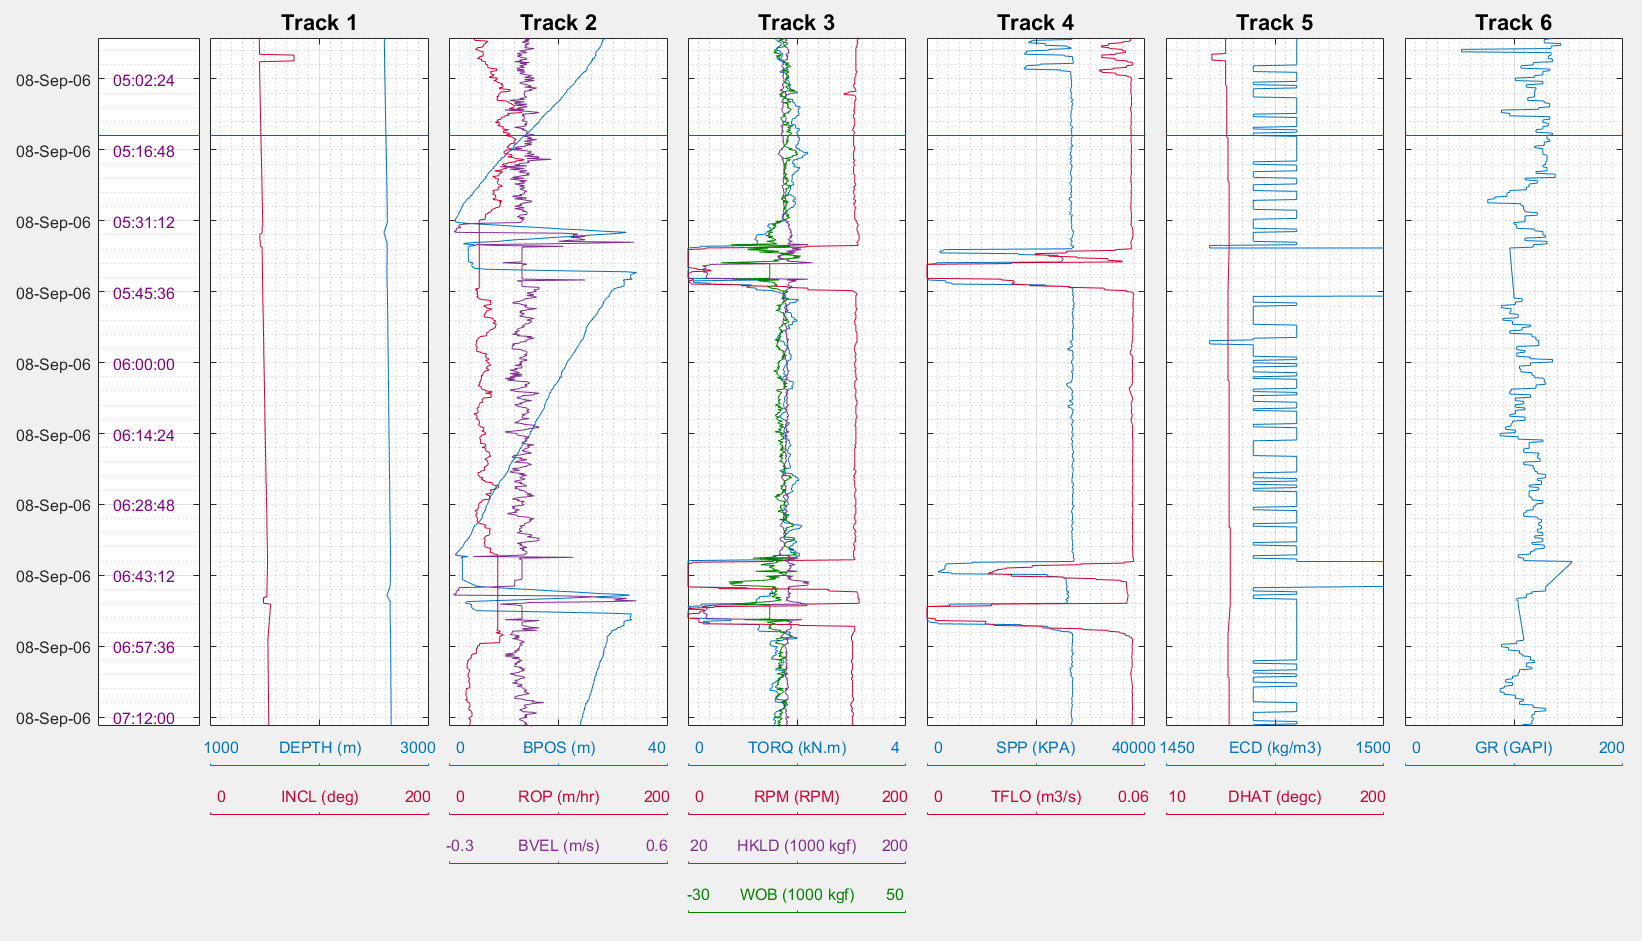
\includegraphics[width=\textwidth]{example1.PNG}
\caption{Curves plotted from template $\#1$}
\end{figure}

\pagebreak
\section{Track template $\#2$}
The plotting template is
\begin{lstlisting}[style=Matlab-editor]
inputTrack = struct(...
    'Name',     {'Track 1','Track 2','Track 3',...
    		'Track 4'},...
    'Curves',   {{'DEPTH','DBTM','BPOS','ROP'},...
                {'TORQ','RPM','HKLD','WOB'},...
                {'SPP','TFLO'},...
                {'GR'}},...
    'XScale',   {'linear','linear','linear',...
    		'linear'});
inputCurves = struct('Name',{'BPOS','ROP'},...
    		     'Min',{0,0});
    
\end{lstlisting}

\noindent This template has 4 tracks:
\begin{enumerate}
\setlength\itemsep{0.1em}
\item Track 1 : Depth, DBTM, BPOS, and ROP
\item Track 2 : Torque, RPM, hookload, and WOB
\item Track 3 : SPP and flow rate
\item Track 4 : Gamma Ray
\end{enumerate}

\noindent The result from this plotting template is shown in figure below
\begin{figure}[H]
\centering
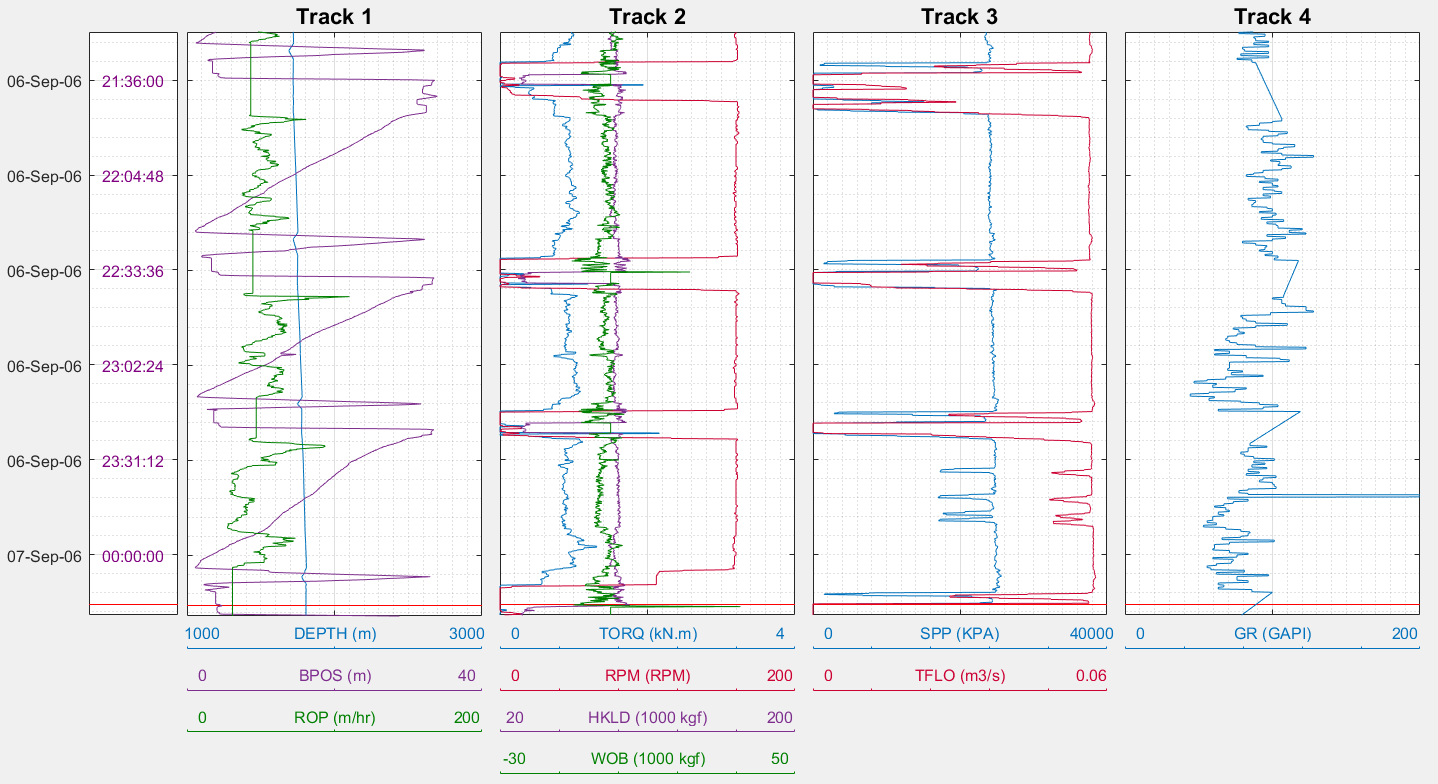
\includegraphics[width=\textwidth]{example2.PNG}
\caption{Curves plotted from template $\#2$}
\end{figure}

\pagebreak
\section{Track template $\#3$}
The plotting template is
\begin{lstlisting}[style=Matlab-editor]
inputTrack = struct(...
    'Name',     {'Track 1','Track 2','Track 3',...
    		'Track 4'},...
    'Curves',   {{'DEPTH','DBTM','BPOS'},...
                {'ROP','BVEL'},...
                {'TORQ','RPM'},...
                {'HKLD','WOB'}},...
    'XScale',   {'linear','linear','linear',...
    		'linear'});
inputCurves = struct('Name',{'BPOS','ROP'},...
    		     'Min',{0,0});
    
\end{lstlisting}

\noindent This template has 4 tracks:
\begin{enumerate}
\setlength\itemsep{0.1em}
\item Track 1 : Depth, DBTM, and BPOS
\item Track 2 : ROP and BVEL
\item Track 3 : Torque and RPM
\item Track 4 : Hookload and WOB
\end{enumerate}

\noindent The result from this plotting template is shown in figure below
\begin{figure}[H]
\centering
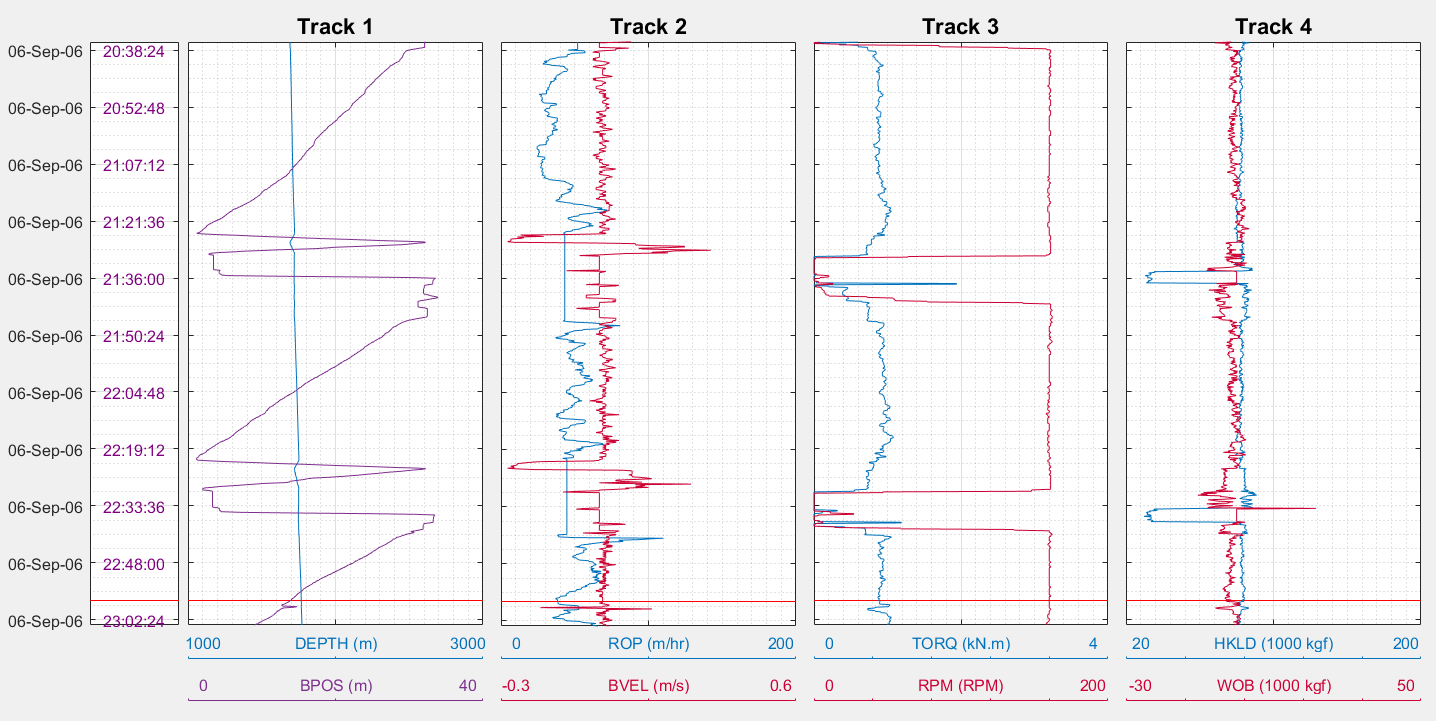
\includegraphics[width=\textwidth]{example3.PNG}
\caption{Curves plotted from template $\#3$}
\end{figure}

\begin{appendices}

\chapter{Parsing process}
\label{ch:parsing}
This chapter discusses a brief details about parsing process within the program. Parsing refers to process to analyze and extract the component parts of raw log file. The parsing program is linked to the log viewer program, but user can also run the parsing program separately. These programs are:
\begin{itemize}
\item \texttt{read$\_$asc$\_$file}, a parsing program for ASC-file. This program can be found in directory \texttt{lib}
\item \texttt{read$\_$csv$\_$file}, a parsing program for CSV-file. This program can be found in directory \texttt{lib}
\item \texttt{read$\_$las$\_$file}, a parsing program for LAS-file. This program can be found in directory \texttt{lib > S4M > Geophysics$\_$3.0}
\end{itemize}
 

\section{The output of parsing}
All types of log file will be processed in the parsing program to return \emph{a standard output} which is a MATLAB \texttt{struct} class type. This output \emph{must} contain fields:
\begin{enumerate}
\setlength\itemsep{0.08em}
\item \texttt{curve$\_$info}, refers to the curve information. This field is a class of \texttt{cell} which contains the curve mnemonic names, units, and description in a successive row.
\item \texttt{curves}, refers to the curves data. This field is a class of \texttt{double}. Each column represent the data value of each curve contained in the log file. The time (and date) string in CSV and ASC file will be converted in a float number based on ISO standard.
\item \texttt{first}, refers to the first depth (or time) in the file
\item \texttt{last}, refers to the last depth (or time) in the file
\item \texttt{step},  represents the actual difference between every successive index value
\item \texttt{units}, refers to the unit of depth (or time) reference
\item \texttt{null}, refers to null values
\item \texttt{wellname}, refers to the well name
\item \texttt{date}, refers to date logged
\end{enumerate}

The following components may or may not be present in the output depends on the availability of these information in the log file
\begin{enumerate}
\setlength\itemsep{0.08em}
\item \texttt{date$\_$time} refers to string of date and time from CSV and ASC file
\item \texttt{company} refers to company name
\item \texttt{field} refers to the well field
\item \texttt{location} refers to the well location
\item \texttt{country} refers to the well location (country)
\item \texttt{service} refers to logging company
\end{enumerate}

\section{Editing and saving the output into MAT-file}
The output from parsing program enables the user to edit the log file easier. For example, if a user want to create a new data curve by combining the existed curves, the user can make a data value easily by editing the field \texttt{curves}.

Another advantage is that the output can also be saved into a MAT-file, a MATLAB file that contains a MATLAB variable. Saving can be performed from the RTDD log viewer application (see \hyperref[ch:save_file]{Chapter \ref{ch:save_file}}) or separately by compiling the program.

\chapter{Standard format of LAS file}
\label{ch:las_std}
LAS is short for Log ASCII standard which holds file specification for various versions of LAS. The specification of LAS file version 2.0 can be found in \url{http://www.cwls.org/wp-content/uploads/2014/09/LAS_20_Update_Jan2014.pdf} and version 3.0 in \url{http://www.cwls.org/wp-content/uploads/2014/09/LAS_3_File_Structure.pdf}.

\section{Troubleshoot for non-standardized LAS file}
The developers noticed that some of the LAS files do not follow the specifications, giving errors during parsing and/or plotting the well log. Within this section, developers listed the most common issues causing errors.

\subsection{Check the well information under $\sim$W section of raw .LAS file}
The problem may arise from:
\begin{itemize}
\item Different units of \textbf{STRT}, \textbf{STOP}, and \textbf{STEP}. The units of these three information must match. In a real-time drilling data, the unit of these information can be in SEC or S.
\item The time index value of \textbf{STRT} and/or \textbf{STOP} is in string format. The supported format is a floating number, while format \{dd/mm/yy\} and/or \{hh:mm:ss\} format is not supported. More detailed information of time-index value: \hyperref[ch:time:index_value]{Chapter \ref{ch:time:index_value}}.
\item Missing \textbf{DATE} information. It is recommended to provide the date information to avoid error during reading time-index value.
\item Make sure each line of well information is delimited with a break or a new line.
\end{itemize}

\subsection{Check the ASCII log data under $\sim$A section of raw .LAS file}
Check the time-reference data. The parsing program only support time-reference data in floating numbers and does not support time data in string format, such as in \{dd/mm/yy\} or \{hh:mm:ss\}. More detailed information of time index-value format: \hyperref[ch:time:index_value]{Chapter \ref{ch:time:index_value}}.

\subsection{Time-index value format}
\label{ch:time:index_value}
The time index is the most crucial information within the real-time log file, thus the formats must be correct. All of the time-index value information must be written in a floating number format, while the string format is not supported. In order to get a floating number of time, usually the time information is encoded based on the standard format. There are wide ranges of standard format on timestamp, but the most formats used in real-time drilling data are UNIX time, GPS epoch time, ISO calendar. 

The log viewer program is designed \ul{based on proleptic ISO calendar} format, but still can process other time-index format. If time-index value is based on UNIX time and GPS epoch time, user must provide the \textbf{DATE} under the well information section, or else the program will give an error. Other standard formats beside UNIX time, GPS epoch time, and ISO calendar are not supported within the program. An example of GPS epoch time-index well log can be found in well 30/3 - A-5 B.


\subsection{Troubleshoot for time index value in string format}
The developer created an additional program to fix the .LAS file of which time-index values are in string format. This additional program must be run separately because it does not linked in the log viewer program. The program is \texttt{fix$\_$las$\_$time$\_$date.m} and can be found in \texttt{lib} directory.

\pagebreak
Below is the example of non-standardized LAS file with wrong format of time and date. The highlighted parts indicates parts that are not following the standard format and required to be fixed.

\begin{mdframed}[backgroundcolor=gray!10]
~Well Information Block
\begin{table}[H]
\begin{tabu} to 1\textwidth {X[l] X[2,r] X[2,l]}
$\#$MNEM.UNIT&                   Data Type& :Information\\
----------- & ---------------&-------------\\
  STRT.\hl{\:\:\:\:\:}     & \hl{09-AUG-2006 13:13:05} &: START INDEX     	\\              
  STOP.\hl{\:\:\:\:\:}     & \hl{09-AUG-2006 13:14:25} &: STOP INDEX       	\\            
  STEP.\hl{SEC}       &    10.0000 &: STEP                   	\\       
  NULL.          &    -999.25 &: NULL VALUE              	\\      
  COMP.    & Conoco Phillips  &: COMPANY               		\\        
  WELL.    &        2/4X-04B  &: WELL                    	\\      
   FLD.    &         Ekofisk  &: FIELD                  	\\       
   LOC.    &                  &: LOCATION                	\\      
  PROV.    &                  &: PROVINCE                 	\\     
  CNTY.    &                  &: COUNTY                   	\\     
  STAT.    &                  &: STATE                     	\\    
  CTRY.    &          Norway  &: COUNTRY                  	\\     
  SRVC.    &    Schlumberger  &: SERVICE COMPANY          	\\     
  DATE.    &       09-AUG-2006 13:13:05 &: LOG DATE        	\\              
   UWI.    &                  &: UNIQUE WELL ID            	\\    
   API.    &                  &: API NUMBER  	
\end{tabu}
\end{table}
\noindent ~ Curve Information Block \\
$\#$
\begin{table}[H]
\begin{tabu} to 1\textwidth {X[l] X[2,l] X[2,l]}   
$\#$MNEM.UNIT &                    &: Curve Description 	\\
$\#$--------- &                    & --------------------	\\
\hl{TIME} &	    .\hl{HHMMSS}	       &: 			\\
\hl{DATE} &    .\hl{D}		       &: 			\\
DEPT &       .FT               &: Bit Depth 2hz                 \\                                
BVEL &       .FT/S             &: Block Velocity 2hz            \\                                  
BPOS &       .FT               &: Block Position 2hz            \\                                  
ROP5 &       .F/HR              &: 5ft ROP 2hz                  \\                                   

\end{tabu}
\end{table}
                                     
\noindent $\#$\\
~Parameter Information Block \\
$\#$MNEM.UNIT                       Value:Description\\
$\#$-----------------------------------------------------------\\
$\#$
\noindent ~Other Information Block\\ $\#$
\begin{table}[H]
\begin{tabu} to 1\textwidth {X[1.5,l] X[1.5,l] X[l] X[l] X[l] X[l]}
~A TIME  &      DATE   &     DEPT    &    BVEL  &      BPOS    &    ROP5  \\
\hl{13:13:05} & \hl{09-Aug-06}   & 11966.73       & 0.00  &     89.07  &   -999.25   \\ 
\hl{13:13:15} & \hl{09-Aug-06}   & 11966.73    & 2493.07  &     89.07  &   -999.25   \\ 
\hl{13:13:25} & \hl{09-Aug-06}   & 11966.73       & 0.00  &     89.07  &   -999.25   \\ 
\hl{13:13:35} & \hl{09-Aug-06}   & 11966.73       & 0.00  &     89.07  &   -999.25   \\ 
\hl{13:13:45} & \hl{09-Aug-06}   & 11966.73       & 0.00  &     89.07  &   -999.25   \\ 
\hl{13:13:55} & \hl{09-Aug-06}   & 11966.73       & 0.00  &     89.07  &   -999.25   \\ 
\hl{13:14:05} & \hl{09-Aug-06}   & 11966.73       & 0.00  &     89.07  &   -999.25   \\ 
\hl{13:14:15} & \hl{09-Aug-06}   & 11966.73     & 0.00    &   89.07    & -999.25   \\ 
\hl{13:14:25} & \hl{09-Aug-06}   & 11966.73     & 0.00    &   89.07    & -999.25   

\end{tabu}
\end{table}
\end{mdframed}

By correction from \texttt{fix$\_$las$\_$time$\_$date.m}, the result will look like following result.

\begin{mdframed}[backgroundcolor=gray!10]
~Well Information Block
\begin{table}[H]
\begin{tabu} to 1\textwidth {X[l] X[2,r] X[2,l]}
$\#$MNEM.UNIT&                   Data Type& :Information\\
----------- & ---------------&-------------\\
  STRT.S   	& 0		&: START INDEX     	\\              
  STOP.S     	&  80&: STOP INDEX       	\\            
  STEP.S       	&    10.0000 &: STEP                   	\\       
  NULL.          &    -999.25 &: NULL VALUE              	\\      
  COMP.    & Conoco Phillips  &: COMPANY               		\\        
  WELL.    &        2/4X-04B  &: WELL                    	\\      
   FLD.    &         Ekofisk  &: FIELD                  	\\       
   LOC.    &                  &: LOCATION                	\\      
  PROV.    &                  &: PROVINCE                 	\\     
  CNTY.    &                  &: COUNTY                   	\\     
  STAT.    &                  &: STATE                     	\\    
  CTRY.    &          Norway  &: COUNTRY                  	\\     
  SRVC.    &    Schlumberger  &: SERVICE COMPANY          	\\     
  DATE.    &       09-AUG-2006 13:13:05 &: LOG DATE        	\\              
   UWI.    &                  &: UNIQUE WELL ID            	\\    
   API.    &                  &: API NUMBER  	
\end{tabu}
\end{table}
\noindent ~ Curve Information Block \\
$\#$
\begin{table}[H]
\begin{tabu} to 1\textwidth {X[l] X[2,l] X[2,l]}   
$\#$MNEM.UNIT &                    &: Curve Description 	\\
$\#$--------- &                    & --------------------	\\
ETIM &	    	.S	       	  &: Elapsed Time			\\
DEPT &       	.FT               &: Bit Depth 2hz                 \\                                
BVEL &       	.FT/S             &: Block Velocity 2hz            \\                                  
BPOS &       	.FT               &: Block Position 2hz            \\                                  
ROP5 &       	.F/HR             &: 5ft ROP 2hz                  \\                                   

\end{tabu}
\end{table}
                                     
\noindent $\#$\\
~Parameter Information Block \\
$\#$MNEM.UNIT                       Value:Description\\
$\#$-----------------------------------------------------------\\
$\#$
\noindent ~Other Information Block\\ $\#$
\begin{table}[H]
\begin{tabu} to 1\textwidth { X[1.5,l] X[l] X[l] X[l] X[l]}
~A TIME  &      DEPT    &    BVEL  &      BPOS    &    ROP5  \\
0   & 11966.73       & 0.00  &     89.07  &   -999.25   \\ 
10  & 11966.73       & 2493.07  &     89.07  &   -999.25   \\ 
20  & 11966.73       & 0.00  &     89.07  &   -999.25   \\ 
30  & 11966.73       & 0.00  &     89.07  &   -999.25   \\ 
40  & 11966.73       & 0.00  &     89.07  &   -999.25   \\ 
50  & 11966.73       & 0.00  &     89.07  &   -999.25   \\ 
60  & 11966.73       & 0.00  &     89.07  &   -999.25   \\ 
70  & 11966.73       & 0.00    &   89.07    & -999.25   \\ 
80  & 11966.73       & 0.00    &   89.07    & -999.25   
\end{tabu}
\end{table}
\end{mdframed}


\chapter{Standard format of CSV file}
\label{ch:csv_std}
This chapter discusses the standard format for CSV-file to be able parsed by parsing program. CSV file is a \emph{comma-separated value} file. In general. CSV-file has two main sections, they are curve information and log data section.

\begin{figure}[ht]
\centering
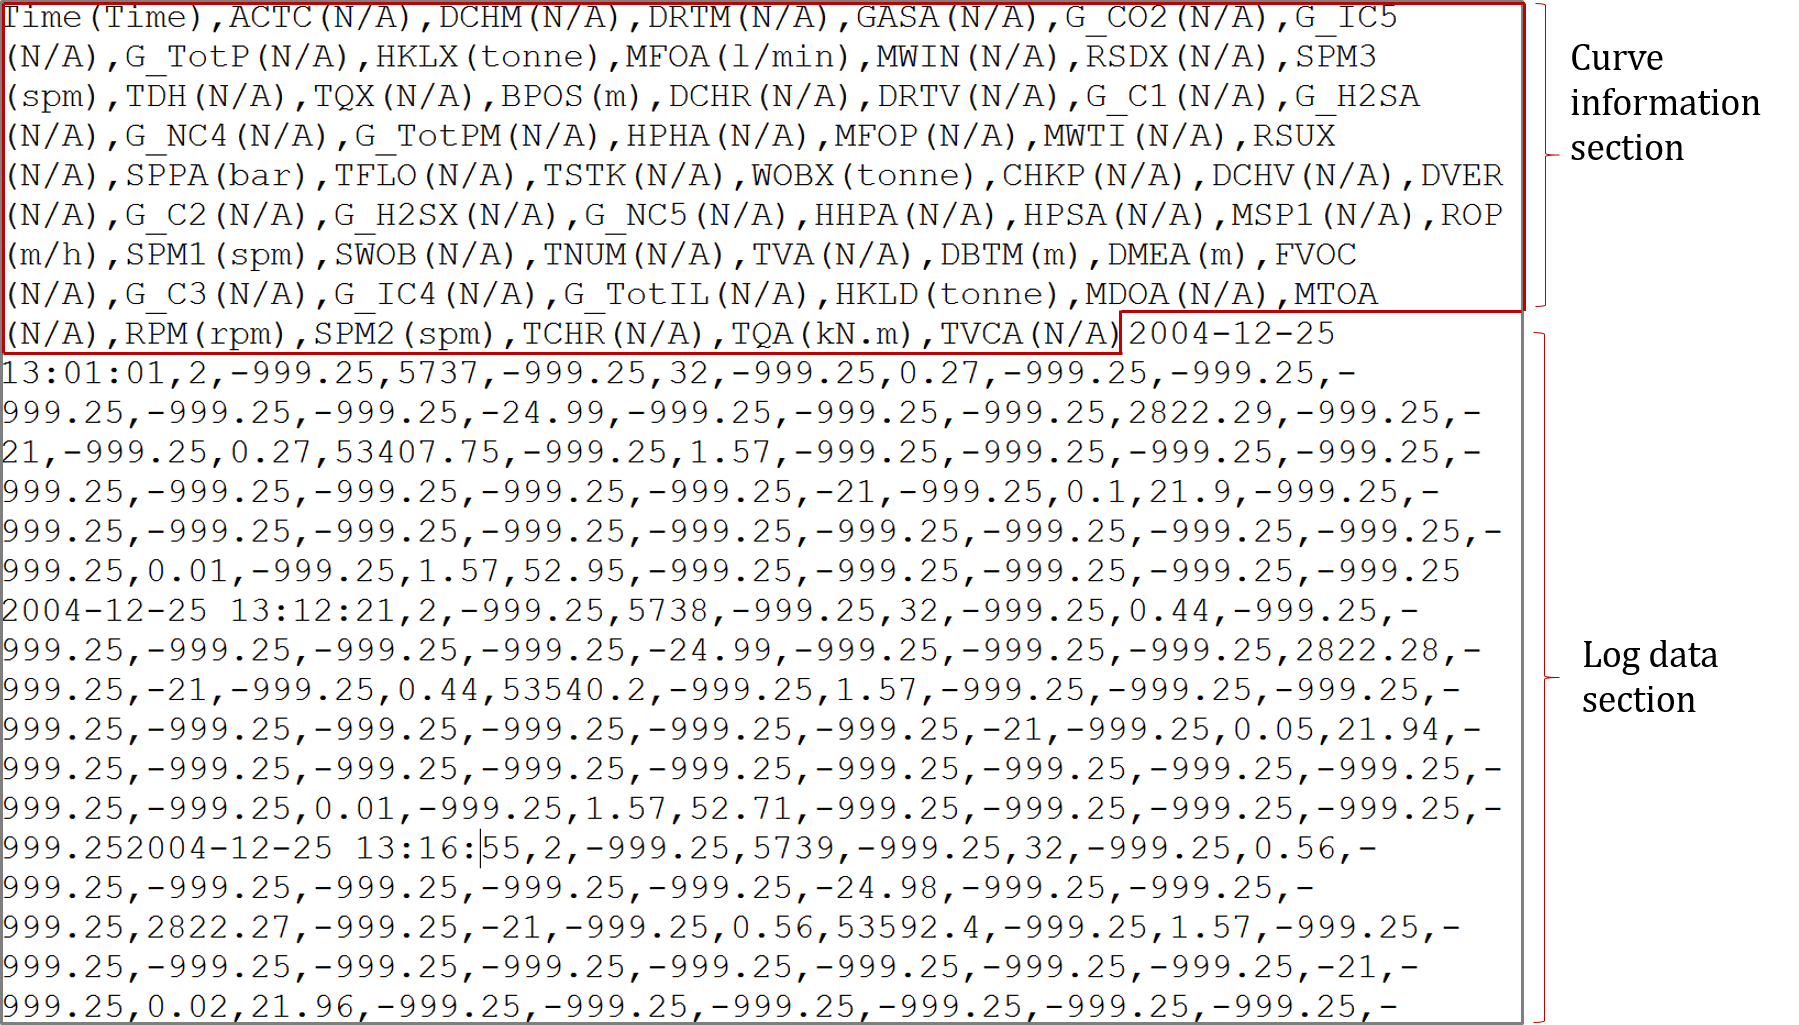
\includegraphics[width=\textwidth]{csv_example.png}
\caption{Example of CSV-file and the sections}
\end{figure}


\section{Well information section}
Log file with .csv file does not have well information section. However some parameters are determined automatically within the parsing program in accordance with the parsing output.

\section{Curve information section}
The curve information is one line which located at the \emph{first} line of the file and contains the mnemonic name and unit of the curves. The curve unit is written next to each curve mnemonic name and it must be begin and ended with parentheses ((..)). The delimiter of each curve information is comma (,). The curve information must be started with \textbf{TIME}.
\paragraph{}
\begin{wrapfigure}[3]{l}{0.08\textwidth}
\vspace{-15pt}

\includegraphics[scale=0.08]{hand_point.png}
\end{wrapfigure}
\noindent\textbf{Attention:} It is \emph{important} to provide the unit of \textbf{TIME} curve. If there is no \textbf{TIME} unit provided, the time string is assumed following format {\color{violet}yyyy-mm-dd HH:MM:SS} by default.

\begin{figure}[ht]
\centering
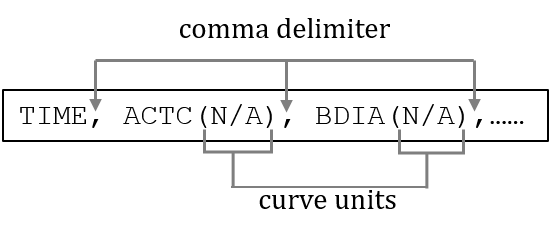
\includegraphics[width=0.5\textwidth]{csv_curve_info_1.png}
\caption{Example of CSV-file curve information and delimiters}
\end{figure}

\section{Log data section}
In each line, the value of each curve is delimited by comma. Unless the \textbf{TIME} data, the rest of log data \emph{must be in float format}.
\pagebreak
\section{Example of standardized CSV-file}
The example of standardized CSV-file to be able parsed by the program is shown below.
\begin{mdframed}[backgroundcolor=gray!10]
\raggedright
\texttt{\seqsplit{%
Time(yyyy-mm-dd \: HH:MM:SS),ACTC(N/A),DCHM(N/A),DRTM(N/A),GASA(N/A),G$\_$CO2(N/A),G$\_$IC5(N/A),G$\_$TotP(N/A),HKLX(tonne),MFOA(l/min)\\
2004-12-25 \: 13:01:01,2,-999.25,5737,-999.25,32,-999.25,0.27,-999.25,-999.25
2004-12-25 \: 13:12:21,2,-999.25,5738,-999.25,32,-999.25,0.44,-999.25,-999.25
2004-12-25 \: 13:16:55,2,-999.25,5739,-999.25,32,-999.25,0.56,-999.25,-999.25
2004-12-25 \: 13:37:43,2,-999.25,5741,-999.25,32,-999.25,0.62,-999.25,-999.25
2004-12-25 \: 14:15:36,3,5735,-999.25,-999.25,-999.25,-999.25,-999.25,-999.25}}
\end{mdframed}

\chapter{Standard format of ASC-file}
\label{ch:asc_std}
The supported format of ASC-file which can be parsed by the programs is discussed within this chapter. ASC-file contains ASCII text format and has 3 sections: well information, curve information, and log data section.

\begin{figure}[ht]
\centering
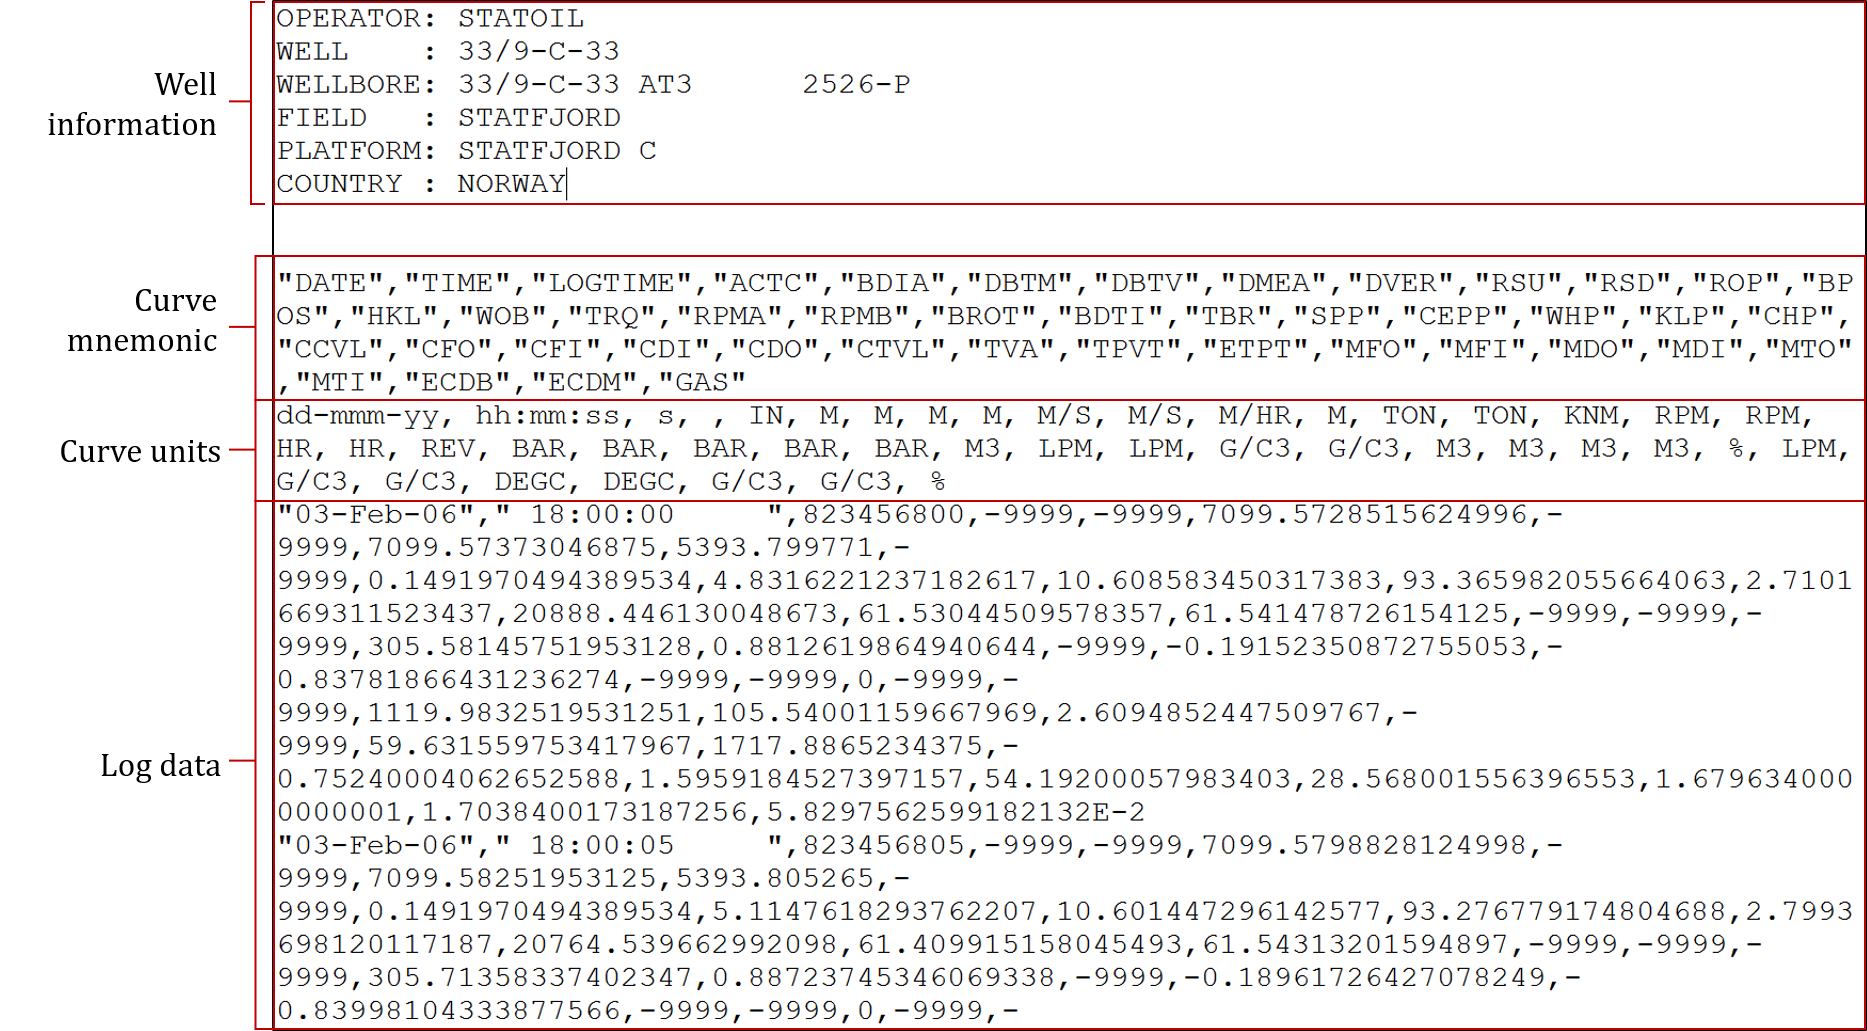
\includegraphics[width=\textwidth]{asc_example.png}
\caption{Example of ASC-file and the sections}
\end{figure}

\section{Well information section}
The well information section is located at the first line of ASC-file. This section is not mandatory and may filled with information similar to well information section of LAS-file. The delimiter of the well information is colon.

In case the ASC-file contains well information, the information can contain:
\begin{enumerate}
\TabPositions{2cm}
\setlength\itemsep{0.1em}
\item \texttt{WELL} \tab{\texttt{: <value/name>}, refers to well name}
\item \texttt{COMP} \tab{\texttt{: <value/name>}, refers to company name}
\item \texttt{FIELD} \tab{\texttt{: <value/name>}, refers to the field name}
\item \texttt{COUNTRY} \tab{\texttt{: <value/name>}, refers to country of the well location}
\item \texttt{STRT} \tab{\texttt{: <value/name>}, refers to the start time}
\item \texttt{STOP} \tab{\texttt{: <value/name>}, refers to the stop time}
\item \texttt{STEP} \tab{\texttt{: <value/name>}, refers to the actual difference between every successive index value}
\item \texttt{NULL} \tab{\texttt{: <value/name>}, refers to null values}
\item \texttt{DATE} \tab{\texttt{: <value/name>}, refers to the date of logging operation}
\end{enumerate}

\noindent The last five well information will calculated or determined automatically by the parsing program in case these information are not provided in the file. 


\section{Curve information section}
Both curves mnemonic names and units must be begin and ended by quotation mark("). The delimiter between each curve mnemonic name and unit is comma (,). The curve units are written directly one line after the mnemonic names line. The curve information must contain and begin with \textbf{DATE}and \textbf{TIME}.
\begin{figure}[ht]
\centering
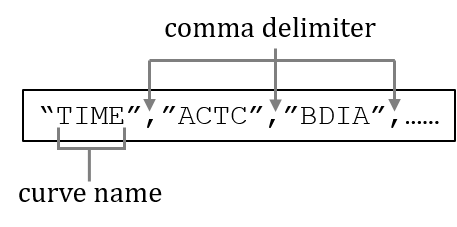
\includegraphics[width=0.45\textwidth]{asc_curve_info_1.png}
\caption{Example of ASC-file curve mnemonic names}
\end{figure}

\begin{wrapfigure}[4]{l}{0.08\textwidth}
\vspace{-15pt}

\includegraphics[scale=0.08]{hand_point.png}
\end{wrapfigure}
\noindent\textbf{Attention:} It is \emph{important} to provide the unit of \textbf{DATE} and \textbf{TIME} curve. If there are no \textbf{DATE} and \textbf{TIME} unit provided, the time string is assumed following format {\color{violet}dd-mmm-yy HH:MM:SS} by default.


\section{Log data section}
In each line, the value of each curve is delimited by comma. Unless the \textbf{DATE} and \textbf{TIME} data, the rest of log data \emph{must be in float format}.

\section{Example of standardized ASC-file}
The example of standardized ASC-file to be able parsed by the program is shown below.

\begin{mdframed}[backgroundcolor=gray!10]
\raggedright\texttt{%
WELL 	: 33/XX-X-XX \\
COMP 	: COMPX \\
FIELD 	: FIELD X \\
COUNTRY : NORWAY \\
\paragraph*{}
\noindent \seqsplit{"DATE","TIME","LOGTIME","ACTC","BDIA","DBTM","DBTV","DMEA","DVER","RSU"\\
dd-mmm-yy, hh:mm:ss, s, , IN, M, M, M, M, M/S\\
"01-Jan-07"," 17:00:00 ",852138000,-9999,-9999,4516.958984375,-9999,4595.0146484375,1191.0538890000003,-9999
"01-Jan-07"," 17:00:05 ",852138005,-9999,-9999,4516.958984375,-9999,4595.0146484375,1191.0538890000003,-9999
"01-Jan-07"," 17:00:10 ",852138010,-9999,-9999,4516.958984375,-9999,4595.0146484375,1191.0538890000003,-9999
"01-Jan-07"," 17:00:15 ",852138015,-9999,-9999,4516.958984375,-9999,4595.0146484375,1191.0538890000003,-9999
"01-Jan-07"," 17:00:20 ",852138020,-9999,-9999,4516.958984375,-9999,4595.0146484375,1191.0538890000003,-9999}}
\end{mdframed}

\end{appendices}
\end{document}
